% \section{Índice}
%     \begin{frame}{}
%     \begin{enumerate}
%         \item Propiedades de dos segmentos. \bigskip
%         \item Intersección de un conjunto de segmentos. \bigskip
%         %\item Envoltura convexa: Método de Graham. \bigskip
%         \item Los dos puntos más cercanos.
%     \end{enumerate}
%     \end{frame}
    
\section{Dos segmentos}
\subsection{Propiedades básicas}
    
    \frame{\sectionpage}
    
    \begin{frame}{Producto vectorial}
    \centering
    \begin{tikzpicture}[scale=0.25]
        \draw[->,>=Latex,thick,orange] (0,0) node[left] {$P_0$} -- (0,7.5) node[left] {$P_2$};
        \draw[->,>=Latex,orange, very thick] (0,0) -- (3.75,5.625) node[right] {$P_1$};
        \draw[->,>=Latex,dashed,thick] (2.5,3.75) arc (60:90:5) node[left] {antihorario};
        % \node at (0,-1) {$\overrightarrow{P_0P_1}\times\overrightarrow{P_0P_2}>0$};
    
    \begin{scope}[xshift=15cm]
        \draw[->,>=Latex,thick,orange] (0,0) node[right] {$P_0$} -- (0,7.5) node[right] {$P_2$};
        \draw[->,>=Latex,orange, very thick] (0,0) -- (-3.75,5.625) node[left] {$P_1$};
        \draw[->,>=Latex,dashed,thick] (-2.5,3.75) arc (120:90:5) node[right] {horario};
        % \node at (0,-1) {$\overrightarrow{P_0P_1}\times\overrightarrow{P_0P_2}<0$};
    \end{scope}
    
    \begin{scope}[xshift=30cm]
        \node[orange,align=center,draw,rounded corners=3pt,thick,minimum width=3cm] at (0,4) {\fancyfont ANTIHORARIO \\\fancyfont HORARIO};
    \end{scope}
    
    \begin{scope}[yshift=-11cm]
        \draw[->,>=Latex,thick,dashed] (0,0) node[left,orange] {$P_0$} -- (0,7.5);
        \draw[->,>=Latex,orange,very thick] (0,0) -- (3.75,5.625) node[right] {$P_1$};
        \draw[->,>=Latex,orange,very thick] (3.75,5.625) -- (0,7.5) node[left] {$P_2$};
        \node at (0,-4) {$\overrightarrow{P_0P_1}\times\overrightarrow{P_0P_2}>0$};
        \node[left] at (0,3.75) {izquierda};
    
    \begin{scope}[xshift=15cm]
        \draw[->,>=Latex,thick,dashed] (0,0) node[right,orange] {$P_0$} -- (0,7.5);
        \draw[->,>=Latex,orange,very thick] (0,0) -- (-3.75,5.625) node[left] {$P_1$};
        \draw[->,>=Latex,orange,very thick] (-3.75,5.625) -- (0,7.5) node[right] {$P_2$};
        \node at (0,-4) {$\overrightarrow{P_0P_1}\times\overrightarrow{P_0P_2}<0$};
        \node[right] at (0,3.75) {derecha};
    \end{scope}
    
    \begin{scope}[xshift=30cm]
        \node[orange,align=center,draw,rounded corners=3pt,thick,minimum width=3cm] at (0,4) {\fancyfont IZQUIERDA \\\fancyfont DERECHA};
    \end{scope}
    \end{scope}
    \end{tikzpicture}
    \end{frame}
    
    \begin{frame}{Intersección de dos segmentos}
    \centering
    \begin{tikzpicture}[scale=0.4]
        \draw[->,>=Latex,orange,very thick] (-1,0) node[inner sep=0] (Q0) {} -- (5,7.5) node[inner sep=0] (Q1) {};
        \draw[->,>=Latex,orange,very thick] (-2,5) node[inner sep=0] (P0) {} -- (4,2) node[inner sep=0] (P1) {};
        \node[left,orange] at (P0) {$P_0$};
        \node[right,orange] at (P1) {$P_1$};
        \node[left,orange] at (Q0) {$Q_0$};
        \node[right,orange] at (Q1) {$Q_1$};
        
        \draw[->,>=Latex,thick] (Q0) -- (P0);
        \draw[->,>=Latex,thick] (Q0) -- (P1);
        \draw[->,>=Latex,thick,dashed] plot [smooth] coordinates {(-1.5,2.5) (-0.5,2.5) (0.1,1.4)};
        \draw[->,>=Latex,thick,dashed] plot [smooth] coordinates {(0.1,1.4) (0.75,1.7) (1.5,1)};
    
    \begin{scope}[xshift=12cm]
        \draw[->,>=Latex,orange,very thick] (-1,0) node[inner sep=0] (Q0) {} -- (5,7.5) node[inner sep=0] (Q1) {};
        \draw[->,>=Latex,orange,very thick] (-2,5) node[inner sep=0] (P0) {} -- (4,2) node[inner sep=0] (P1) {};
        \node[left,orange] at (P0) {$P_0$};
        \node[right,orange] at (P1) {$P_1$};
        \node[left,orange] at (Q0) {$Q_0$};
        \node[right,orange] at (Q1) {$Q_1$};
        
        \draw[->,>=Latex,thick] (P0) -- (Q0);
        \draw[->,>=Latex,thick] (P0) -- (Q1);
        \draw[->,>=Latex,thick,dashed] plot [smooth] coordinates {(-1.5,2.5) (-0.5,2.5) (0,4)};
        \draw[->,>=Latex,thick,dashed] plot [smooth] coordinates {(0,4) (1,4.75) (1,6)};
        
        \node at (8.5,5) {\Huge\cmark};
        \end{scope}
    \end{tikzpicture}
    
    \bigskip
    
    \begin{tikzpicture}[scale=0.4,rotate=-45]
        \draw[->,>=Latex,orange,very thick] (-1,0) node[inner sep=0] (Q0) {} -- (5,6.5) node[inner sep=0] (Q1) {};
        \draw[->,>=Latex,orange,very thick] (-2,5) node[inner sep=0] (P0) {} -- (0.5,5) node[inner sep=0] (P1) {};
        \node[left,orange] at (P0) {$P_0$};
        \node[right,orange] at (P1) {$P_1$};
        \node[left,orange] at (Q0) {$Q_0$};
        \node[right,orange] at (Q1) {$Q_1$};
        
        \draw[->,>=Latex,thick] (Q0) -- (P0);
        \draw[->,>=Latex,thick] (Q0) -- (P1);
        \draw[->,>=Latex,thick,dashed] plot [smooth] coordinates {(-1.5,2.5) (-0.5,2.5) (0.1,1.3)};
        \draw[->,>=Latex,thick,dashed] plot [smooth] coordinates {(0.5,1.75) (0.4,2.25) (0,3)};
        
        \node at (7.5,11.5) {\Huge\xmark};
    \end{tikzpicture}
    \end{frame}
    
    % \begin{frame}{Intersección de dos segmentos}
    % \centering
    % \begin{tikzpicture}[scale=0.5]
    %     \draw[->,>=Latex,orange,very thick] (-1,0) node[inner sep=0] (Q0) {} -- (5,7.5) node[inner sep=0] (Q1) {};
    %     \draw[->,>=Latex,orange,very thick] (-2,5) node[inner sep=0] (P0) {} -- (1.3,2.85) node[inner sep=0] (P1) {};
    %     \node[left,orange] at (P0) {$P_0$};
    %     \node[right,orange] at (P1) {$P_1$};
    %     \node[left,orange] at (Q0) {$Q_0$};
    %     \node[right,orange] at (Q1) {$Q_1$};
    
    % \begin{scope}[xshift=12.5cm]
    %     \node at (-1,0) {};
    %     \draw[->,>=Latex,orange,very thick] (1.8,3.5) node[inner sep=0] (Q0) {} -- (5,7.5) node[inner sep=0] (Q1) {};
    %     \draw[->,>=Latex,orange,very thick] (-2,5) node[inner sep=0] (P0) {} -- (1.3,2.85) node[inner sep=0] (P1) {};
    %     \node[left,orange] at (P0) {$P_0$};
    %     \node[below,orange] at (P1) {$P_1$};
    %     \node[right,orange] at (Q0) {$Q_0$};
    %     \node[right,orange] at (Q1) {$Q_1$};
    % \end{scope}
    % \end{tikzpicture}
    % \end{frame}
    
    \section{Intersección de segmentos}
    \subsection{Barrido horizontal}
    
    \frame{\sectionpage}
    
    % \begin{frame}{Consideraciones}
    % \begin{itemize}
    %     \item Complejidad $\mathcal{O}(nlog(n))$.
    %     \item Solo encontramos una intersección, no todas. 
    %     \begin{itemize}
    %         \item Para encontrar todas se necesita $\mathcal{O}(n^2)$.
    %     \end{itemize}
    %     \item No hay segmentos verticales y no hay intersecciones triples.
    %     \begin{itemize}
    %         \item Fácilmente arreglable.
    %     \end{itemize}
    % \end{itemize}
    % \end{frame}
    
    
    \begin{frame}{Barrido}
    \begin{center}
    
    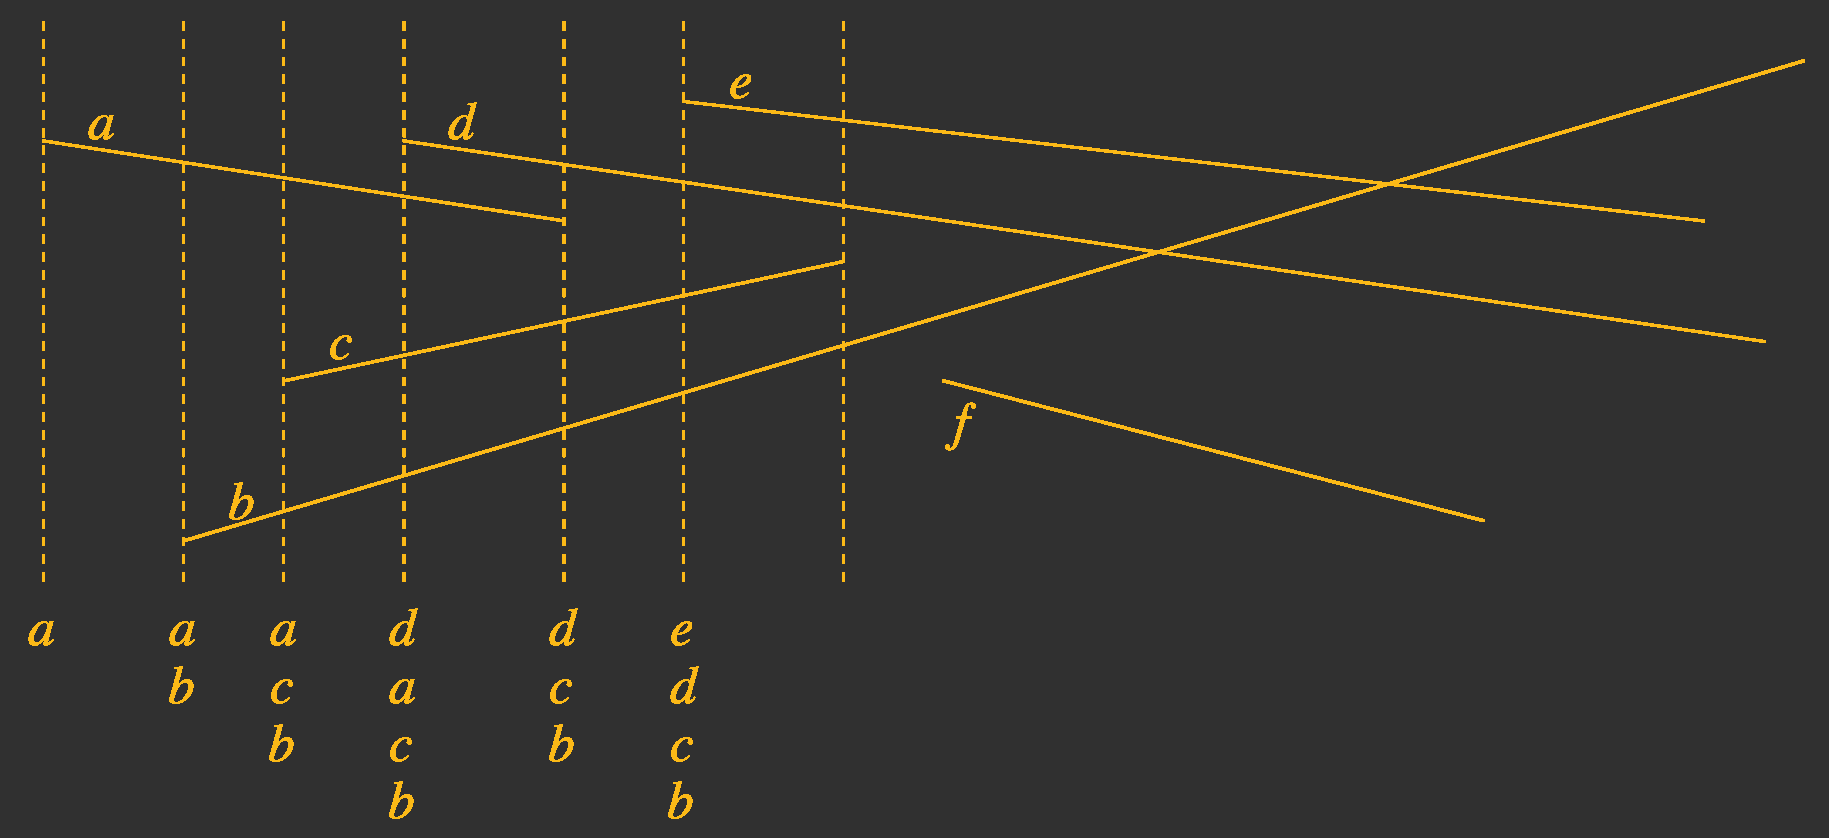
\includegraphics[width=\textwidth]{img/bosweep.png}
    % \begin{tikzpicture}
    % \foreach\i in {0,1,2.2,4.25,5.5} {
    %     \draw[dashed,orange] (\i,0.75) -- (\i,5);
    % }
    % \draw[orange,thick] (0,1) node [above right=4pt] {$a$} -- (10,4);
    % \draw[orange,thick] (1,2) node [above right=4pt] {$b$} -- (5.5,3.25);
    % \draw[orange,thick] (2.2,4.25) node [above right] {$c$} -- (10,2.75);
    % \draw[orange,thick] (4.25,4.5) node [above right] {$d$} -- (9.5,3.5);
    % \draw[orange,thick] (6.5,2) node [above right] {$e$} -- (9,1);
    % \end{tikzpicture}
    
    \bigskip
    
    $P_0=\{x_0,\ C,\ y_0,\ a\}$ \quad $P_1=\{x_1,\ C,\ y_1,\ b\}$ \quad $\cdots$% $P_2=\{x_2,\ C,\ y_2,\ c\}$
    
    % $P_3=\{x_3,\ F,\ y_3,\ d\}$ \quad $P_4=\{x_5,\ F,\ y_5,\ b\}$
    
    % $P_3=\{x_3,\ C,\ y_3,\ d\}$ \quad $P_4=\{x_4,\ F,\ y_4,\ a\}$ \quad $P_5=\{x_5,\ C,\ y_5,\ e\}$
    
    \end{center}
    \end{frame}
    
    \begin{frame}{Barrido}{}
    {\color{orange}---} Ordeno los puntos.\\
    {\color{orange}---} Recorro los puntos:
    \begin{itemize}
        \item ?`Es comienzo de un nuevo segmento?
        \begin{itemize}
        \item Encuentro su lugar con respecto al resto de comienzos.
        \item ?`Interseca con el de arriba o con el de abajo?
            \begin{itemize}
            \item Vistazo a sus puntos finales.
            \end{itemize}
        \end{itemize}
        \item ?`Es final de un segmento?
        \begin{itemize}
        \item Encuentro dónde está su comienzo y dejo su hueco.
        \item ?`Intersecan el de arriba y el de abajo del hueco?
            \begin{itemize}
            \item Vistazo a sus puntos finales.
            \end{itemize}
        \end{itemize}
    \end{itemize}
    \end{frame}
    
    \begin{frame}{Complejidad}{}
    {\color{orange}---} Ordeno los puntos. {\color{orange}$\mathcal{O}(nlog(n))$}\\
    {\color{orange}---} Recorro los puntos: {\color{orange}$\mathcal{O}(nlog(n))$ \quad {\footnotesize($\mathcal{O}(n)*\text{dentro}$)}}
    \begin{itemize}
        \item ?`Es comienzo de un nuevo segmento?
        \begin{itemize}
        \item Encuentro su lugar con respecto al resto de comienzos. {\color{orange}$\mathcal{O}(log(n))$}
        \item ?`Interseca con el de arriba o con el de abajo?
            \begin{itemize}
            \item Vistazo a sus puntos finales. {\color{orange}$\mathcal{O}(1)$}
            \end{itemize}
        \end{itemize}
        \item ?`Es final de un segmento?
        \begin{itemize}
        \item Encuentro dónde está su comienzo y dejo su hueco. {\color{orange}$\mathcal{O}(log(n))$}
        \item ?`Intersecan el de arriba y el de abajo del hueco?
            \begin{itemize}
            \item Vistazo a sus puntos finales. {\color{orange}$\mathcal{O}(1)$}
            \end{itemize}
        \end{itemize}
    \end{itemize}
    \end{frame}
    
    \begin{frame}{Complejidad}{}
        \begin{center}
            Buscar, insertar y borrar en $\mathcal{O}(log(n))$:
            
            \bigskip
            
            {\huge\color{orange}Árboles AVL, rojinegros, etc.}
        \end{center}
    \end{frame}
    
\section{Envoltura convexa}
    
    \frame{\sectionpage}
    
    \begin{frame}{Consideraciones}
        \begin{itemize}
            \item Los puntos son únicos.
            \item Hay al menos 3 puntos no colineales.
            \item El método de Graham opera en $\mathcal{O}(nlog(n))$. Hay otros algoritmos:
            \begin{itemize}
                \item Método de Jarvis: $\mathcal{O}(nh)$, con $h$ el tamaño de la solución.
                \item Con búsqueda y poda, se puede llegar a $\mathcal{O}(nlog(h))$.
            \end{itemize}
        \end{itemize}
    \end{frame}
    
    \newcommand{\dotsGraham}{%
    \node[orange,inner sep=1,circle] (P0) at (0,0) {$\bullet$};
	
	\foreach\i in {1,...,10} {
		\node[inner sep=0,circle] (P\i) at (180*\i/11:{sin(\i*\i*8)+3} ) {$\bullet$};
	}
    }
    
    \begin{frame}{Método de Graham}{}
    \centering
\begin{tikzpicture}[scale=0.4]
	\node[inner sep=1,circle] (P0) at (0,0) {$\bullet$};
	
	\foreach\i in {1,...,10} {
		\node[inner sep=0,circle] (P\i) at (180*\i/11:{sin(\i*\i*8)+3} ) {$\bullet$};
	}
	
	\begin{scope}[xshift=10cm]
	\dotsGraham
	\node at (0,-1.5) {$\mathcal{O}(n)$};
	\end{scope}
	
	\begin{scope}[xshift=20cm]
	\dotsGraham
	
	\foreach\i in {1,...,10} {
		\draw[dashed] (P0) -- (P\i);
	}
	\node at (0,-1.5) {$\mathcal{O}(nlog (n))$};
	\end{scope}
\end{tikzpicture}
	
\bigskip
\pause
	
\begin{tikzpicture}[scale=0.4]
	\dotsGraham
	\draw (P0) -- (P1);
	
	\begin{scope}[xshift=10cm]
	\dotsGraham
	\draw (P0) -- (P1) -- (P2);
	\node at (0,-1.5) {?`Izquierda? \cmark};
	\end{scope}
	
	\begin{scope}[xshift=20cm]
	\dotsGraham
	\draw (P0) -- (P1) -- (P2) -- (P3) -- (P4) -- (P5) -- (P6);
	\end{scope}
\end{tikzpicture}
	
    \end{frame}
    
    \begin{frame}{Método de Graham}{}
    \centering
\begin{tikzpicture}[scale=0.4]
	\dotsGraham
	\draw (P0) -- (P1) -- (P2) -- (P3) -- (P4) -- (P5) -- (P6);
	\draw[dashed] (P6) -- (P7);
	\node at (0,-1.5) {!`Derecha! \xmark};
	
	\begin{scope}[xshift=10cm]
	\dotsGraham
	\draw (P0) -- (P1) -- (P2) -- (P3) -- (P4) -- (P5);
	\draw[dashed] (P5) -- (P7);
	\node at (0,-1.5) {!`Derecha! \xmark};
	\end{scope}
	
	\begin{scope}[xshift=20cm]
	\dotsGraham
	\draw (P0) -- (P1) -- (P2) -- (P3) -- (P4);
	\draw (P4) -- (P7);
	\end{scope}
\end{tikzpicture}

\bigskip
\pause

\begin{tikzpicture}[scale=0.4]
	\dotsGraham
	\draw (P0) -- (P1) -- (P2) -- (P3) -- (P4) -- (P7);
	\draw (P7) -- (P8) -- (P9);
	
	\begin{scope}[xshift=10cm]
	\dotsGraham
	\draw (P0) -- (P1) -- (P2) -- (P3) -- (P4) -- (P7) -- (P8) -- (P9);
	\draw[dashed] (P9) -- (P10);
	\node at (0,-1.5) {!`Derecha! \xmark};
	\end{scope}
	
	\begin{scope}[xshift=20cm]
	\dotsGraham
	\draw (P0) -- (P1) -- (P2) -- (P3) -- (P4) -- (P7) -- (P8) -- (P10) -- (P0);
	\end{scope}
\end{tikzpicture}
    \end{frame}
    
\section{Puntos más cercanos}
\subsection{Divide y vencerás}

    \frame{\sectionpage}
        
    
	
	\newcommand{\dotsClose}{%
		\foreach\i in {1,3,...,10} {
			\node[inner sep=1pt,circle,draw,fill] (P\i) at (180*\i/11:{sin(\i*\i*\i*6)+2} ) {};
		}
		\foreach\i in {1,...,4} {
			\node[inner sep=1pt,circle,draw,fill] (Q\i) at (180*\i/5:{sin(\i*\i*\i*6)+3} ) {};
		}
	}
\begin{frame}{Algoritmo}
	\centering
	Guardo los puntos en dos vectores ordenados: por su $x$ y por su $y$.
	
	\bigskip
	
\begin{tikzpicture}[scale=0.4]
\dotsClose

\begin{scope}[xshift=10cm]
	\dotsClose
	\draw (0.1,-0.5)--(0.1,4);
	\draw (-3.1,-0.2) -- (-3.1,-0.5) -- (-0.2,-0.5) node[below,midway] {P$_\text{izq}$} -- (-0.2,-0.2);
	\draw (0.4,-0.2) -- (0.4,-0.5) -- (3.3,-0.5) node[below,midway] {P$_\text{dcha}$} -- (3.3,-0.2);
\end{scope}

\begin{scope}[xshift=20cm]
	\dotsClose
	\draw (0.1,-0.2)--(0.1,4);
	\draw[orange] (P9) node[inner sep=1pt,circle,draw=orange,fill=orange] {} -- (Q4) node[below=8pt,white] {$\delta_\text{izq}$} node[inner sep=1pt,circle,draw=orange,fill=orange] {};
	\draw[orange] (P3) node[inner sep=1pt,circle,draw=orange,fill=orange] {} -- (Q1) node[above=2pt,white] {$\delta_\text{dcha}$} node[inner sep=1pt,circle,draw=orange,fill=orange] {};
	\node[below] at (0.1,-0.5) {$\delta=\min\{\delta_\text{izq},\delta_\text{dcha}\}$};
\end{scope}
\end{tikzpicture}

\bigskip

\begin{tikzpicture}[scale=0.4]
\dotsClose
\draw (0.1,-0.5)--(0.1,4);
\draw[dashed] (0.8,0)--(0.8,4);
\draw[dashed] (-0.6,0)--(-0.6,4);
\draw (-0.6,-0.2) -- (-0.6,-0.5) -- (0.8,-0.5) node[below,midway] {$2\delta$} -- (0.8,-0.2);

\begin{scope}[xshift=10cm]
	\dotsClose
	\draw[dashed] (0.8,0)--(0.8,4);
	\draw[dashed] (-0.6,0)--(-0.6,4);
	\draw[orange] (P7) node[inner sep=1pt,circle,draw=orange,fill=orange] {} -- (P5) node[inner sep=1pt,circle,draw=orange,fill=orange] {};
	\node[below] at (0.1,-0.5) {\xmark};
\end{scope}

\begin{scope}[xshift=20cm]
	\dotsClose
	\draw[orange] (Q4) node[inner sep=1pt,circle,draw=orange,fill=orange] {} -- (P9) node[inner sep=1pt,circle,draw=orange,fill=orange] {};
	\node[below] at (0.1,-0.5) {\cmark};
\end{scope}
\end{tikzpicture}
    \end{frame}
    
    
    \begin{frame}{Algoritmo}{}
    {\color{orange}---} Ordeno los puntos por su $x$ (X) y por su $y$ (Y).\\
    {\color{orange}---} Llamadas recursivas:
    \begin{itemize}
        \item Divido X por la mitad y lo uso para dividir Y.
        \begin{itemize}
        \item Obtengo recursivamente las soluciones de ambas partes. Tomo la menor, $\delta$, como cota superior.
        \item Quedan por comprobar las parejas con un punto en cada mitad.
            \begin{itemize}
            \item Tomo puntos dentro de una franja de $2\delta$ (ordenados por $y$).
            \item Para cada punto de la franja, solo tengo que comprobar máximo sus 7 puntos inferiores más cercanos.
            \end{itemize}
        \end{itemize}
    \end{itemize}
    {\color{orange}---} Caso base cuando $n\leq 3$.
    \end{frame}
    
    \begin{frame}{Complejidad}{}
    {\color{orange}---} Ordeno los puntos por su $x$ (X) y por su $y$ (Y). {\color{orange}$\mathcal{O}(nlog(n))$}\\
    {\color{orange}---} Llamadas recursivas: {\color{orange}$T(n)=2T(\frac{n}{2})+\mathcal{O}(n)\in\mathcal{O}(nlog(n))$}
    \begin{itemize}
        \item Divido X por la mitad y lo uso para dividir Y. {\color{orange}$\mathcal{O}(n)$}
        \begin{itemize}
        \item Obtengo recursivamente las soluciones de ambas partes. Tomo la menor, $\delta$, como cota superior. {\color{orange}$2T(\frac{n}{2})$}
        \item Quedan por comprobar las parejas con un punto en cada mitad.
            \begin{itemize}
            \item Tomo puntos dentro de una franja de $2\delta$ (ordenados por $y$). {\color{orange}$\mathcal{O}(n)$}
            \item Para cada punto de la franja, solo tengo que comprobar máximo sus 7 puntos inferiores más cercanos. {\color{orange}$\mathcal{O}(n)$}
            \end{itemize}
        \end{itemize}
    \end{itemize}
    {\color{orange}---} Caso base cuando $n\leq 3$.
    \end{frame}
    
    \begin{frame}{Complejidad}{}
    \centering
    ?`Por qué solo necesito comprobar 7 puntos?
    
    Esta es la peor situación posible, donde los puntos intermedios son dobles y cada uno pertenece a una mitad:
    
    \bigskip
    \begin{tikzpicture}
	
	\fill[fill=black!25,opacity=0.5] (0,1) rectangle (4,-1);
	
	\draw[dashed,thick] (0,-1.5) -- (0,1.5);
	\draw[thick] (2,-1.5) -- (2,1.5);
	\draw[dashed,thick] (4,-1.5) -- (4,1.5);
	
	\draw[<->,>=Latex] (0,1.25) -- (2,1.25) node[above,midway] {$\delta$};
	\draw[<->,>=Latex] (2,1.25) -- (4,1.25) node[above,midway] {$\delta$};
	\draw[<->,>=Latex] (-0.25,-1) -- (-0.25,1) node[left,midway] {$\delta$};
	
	
	\node[inner sep=2pt,circle,draw=black,fill] at (1.95,-1) {};
	\node[inner sep=2pt,circle,draw=black,fill] at (1.95,1) {};
	\node[inner sep=2pt,circle,draw=black,fill] at (2.05,-1) {};
	\node[inner sep=2pt,circle,draw=black,fill] at (2.05,1) {};
	
	\node[inner sep=2pt,circle,draw=black,fill] at (0,-1) {};
	\node[inner sep=2pt,circle,draw=black,fill] at (0,1) {};
	\node[inner sep=2pt,circle,draw=black,fill] at (4,-1) {};
	\node[inner sep=2pt,circle,draw=black,fill] at (4,1) {};
	
	\end{tikzpicture}
    \end{frame}
    
    